% Beyond Ablation: A Taxonomy of Interventions for Mechanistic Interpretability
% Applied Intelligence (Springer Nature) -- sn-jnl template
%
\documentclass[pdflatex,sn-mathphys-num]{sn-jnl}

%%%% Packages
\usepackage{graphicx}%
\usepackage{amsmath,amssymb}%
\usepackage{booktabs}%
\usepackage{xcolor}%
\hypersetup{hidelinks}%
\usepackage{cleveref}%
\usepackage{bm}%
\usepackage{algorithm}%
\usepackage{algpseudocode}%
%%%%

\begin{document}

\title[Beyond Ablation]{Beyond Ablation:\\A Taxonomy of Interventions for Mechanistic Interpretability}

\author*[1]{\fnm{Dong} \sur{Liu}}\email{liudong@lynu.edu.cn}
\author[2]{\fnm{Caihuan} \sur{Zhang}}

\affil*[1]{\orgdiv{School of Software}, \orgname{Luoyang Normal University}, \orgaddress{\city{Luoyang}, \state{Henan}, \postcode{471934}, \country{China}}}
\affil[2]{\orgdiv{School of Mathematics}, \orgname{Luoyang Normal University}, \orgaddress{\city{Luoyang}, \state{Henan}, \postcode{471934}, \country{China}}}

\abstract{
Ablation --- the complete removal of a model component --- remains the dominant intervention method in mechanistic interpretability (MI). This paper argues that the MI community suffers from an ``ablation bias'': treating a single boundary point of a continuous intervention space as the universal tool for causal analysis.

Drawing on patterns observed across recent MI work, we identify recurring structural limitations of ablation: it is simultaneously (1) computationally wasteful, (2) blind to multi-component synergy, and (3) destructive to representational structure. We propose a formal three-dimensional intervention space defined by information retention, causal granularity, and temporal-spatial scope, and map existing intervention methods onto this manifold.

Through controlled experiments comparing six intervention methods across three standard MI benchmarks on Pythia-1.4B (24 layers, 16 heads, 2048 hidden), we find that different intervention methods disagree on component importance rankings (mean Kendall $\tau = -0.10$), and that zero ablation over-reports component importance by 85\% compared to mean ablation (Kendall $\tau = -0.51$). We replicate these findings on GPT-2 Small (12 layers), confirming qualitative cross-model consistency. Representational health metrics (Activation Preservation Score) reveal silent damage invisible to behavioral metrics alone.

We conclude with actionable guidelines for method selection and a call to action: the MI community needs a standard intervention ontology, analogous to how traditional ML benefits from a taxonomy of evaluation metrics.
}

\keywords{mechanistic interpretability \sep causal intervention \sep ablation \sep activation steering \sep representation analysis}

\maketitle

%%%%%%%%%%%%%%%%%%%%%%%%%%%%%%%%%%%%%%%%%%%%%%%%%%
\section{Introduction}
\label{sec:introduction}

Mechanistic interpretability (MI) is the dominant framework for understanding how neural networks implement specific behaviors~\cite{Olah2020,Elhage2022}. The core methodological pattern is causal intervention: isolate a component (neuron, attention head, or layer), modify its behavior in a controlled way, and observe the downstream effect on model outputs~\cite{Vig2020,Wang2022}.

In practice, this almost always means ablation: setting the component activation to zero, its mean value across a dataset, or a resampled value. Ablation is simple, interpretable, and widely supported by libraries like TransformerLens~\cite{NandaBloom2022}. But is it always the right tool?

This paper examines a pattern we observe across diverse areas of recent MI work, from dictionary learning and circuit analysis to probing and information theory. Several patterns recur across this work:

\textbf{Computational waste:} Full ablation sweeps across layers are expensive. Accuracy-based removal ranking on LLaMA-3-8B takes 4.6 hours versus 8.6 minutes for fast methods~\cite{Hinostroza2026}.

\textbf{Blindness to synergy:} A component can be causally necessary (ablation causes $-0.96$ performance drop) yet causally insufficient: the function is a multi-component collaboration~\cite{Rumbelow2026}.

\textbf{Structural destruction:} Wrecking-ball ablation removes an entire subnetwork, causing the embedding space to collapse~\cite{LehnSchioler2026}.

\textbf{Gratuitous overkill:} In Transformer world models, the residual stream already contains 98.77\% correct digit ranking before the final MLP. The MLP merely amplifies; ablation confirms a known conclusion at unnecessary cost~\cite{KniazevFijalkow2026}.

These are structural consequences of treating a single point in a continuous intervention space as the universal tool. Just as the MI community has recognized that one metric cannot tell the whole story --- Proposition 4 of Hayashi~\cite{Hayashi2026} formally proves that any single marginal metric (entropy, active-code count, mutual information) has a provable blind spot --- we argue that one intervention method cannot answer all causal questions.

Our contributions:
\begin{enumerate}
    \item We identify recurring structural limitation patterns of ablation, illustrated through independently published MI work spanning multiple sub-areas.
    \item We propose a formal three-dimensional intervention space and map existing methods onto this manifold. Zhang and Nanda~\cite{ZhangNanda2023} previously investigated best practices for activation patching, recommending it over ablation; our work extends this by systematically characterizing the full intervention space across six methods and three circuits, and by analyzing representational health with Activation Preservation Score, a dimension that prior work does not address.
    \item We systematically compare six intervention methods across three standard MI benchmarks on two model scales (Pythia-1.4B and GPT-2 Small), revealing substantial method disagreement (mean Kendall $\bar\tau = -0.10$).
    \item We provide actionable guidelines for method selection and a call to action for the community.
\end{enumerate}

\textbf{Scope.} The patterns we discuss are drawn from published work that we take as illustrative of broader trends; we do not claim exhaustive or systematic coverage. The experiments in this paper (Section~\ref{sec:experiments}) provide one empirical instantiation of the method-disagreement phenomenon, validated across two model scales. We encourage future systematic reviews and larger-scale replications to test the generality of our claims.

%%%%%%%%%%%%%%%%%%%%%%%%%%%%%%%%%%%%%%%%%%%%%%%%%%
\section{Related Work}
\label{sec:related}

\subsection{Ablation as the Dominant Intervention Paradigm}

The theoretical foundation for this approach is the causal abstraction framework of~\cite{Geiger2021}, which formalizes when an interpretable high-level model is a valid causal abstraction of a neural network's internal computations. Under this framework, ablation is a necessity test: if removing a component degrades task performance, that component is causally necessary for the behavior. This framework has been extended through interchange interventions and distributed alignment search (Geiger et al., 2023), establishing a rigorous causal semantics for neural circuit analysis.

Building on this foundation,~\cite{Wang2022} identified the Indirect Object Identification (IOI) circuit in GPT-2 Small using activation patching, demonstrating that a sparse set of attention heads implements a specific linguistic capability.~\cite{Conmy2023} scaled this approach with Automated Circuit Discovery (ACDC), which uses recursive ablation pruning to identify minimal circuits with provable faithfulness guarantees.~\cite{Meng2022} introduced causal tracing in ROME, corrupting intermediate activations and measuring recovery to localize factual associations with high spatial precision. These foundational works established ablation as the de facto gold standard in MI, supported by libraries like TransformerLens~\cite{NandaBloom2022} that provide first-class utilities for zero, mean, and resample ablation across any model component.

However,~\cite{Hinostroza2026} recently demonstrated critical limitations of the metrics commonly used to justify ablation targets. They prove theoretically that a layer can exhibit arbitrarily low cosine similarity while remaining crucial to model performance, and show empirically that cosine similarity misclassifies layer importance in 93.8\% of cases (Spearman $\rho = -0.15$ to $-0.46$). More significantly for scalability, full ablation sweeps across all layers of LLaMA-3-8B require 4.6 hours, versus 8.6 minutes for fast approximation methods, a $32\times$ cost premium.

\subsection{The Necessity-Sufficiency Gap}

A growing body of evidence reveals that ablation's fundamental limitation is conceptual, not merely computational: ablation tests causal necessity, not sufficiency. \cite{Rumbelow2026} provides the clearest demonstration through Exemplar Partitioning (EP), an unsupervised method for constructing interpretable feature dictionaries. In instruction-tuned Gemma-2-2B, EP reveals that the refusal direction is causally necessary (ablation causes a $-0.96$ performance drop) yet causally insufficient, because refusal is implemented through multi-component collaboration. Moreover, EP's comparison with SAE features shows that both methods decompose activation space differently, agreeing only on a limited core ($\sim20\%$ of EP regions match an SAE feature at F1 $> 0.5$), highlighting the intervention-poverty of relying on any single method.

\cite{KniazevFijalkow2026} reinforce this finding through a different lens. Analyzing an 8-layer transformer trained on Sudoku, they show that the residual stream already encodes 98.77\% of the correct digit ranking before the final MLP layer. The MLP merely amplifies an existing representation. Ablation of this component confirms a known conclusion at unnecessary experimental cost. This exemplifies the ``gratuitous overkill'' pattern: ablation is used where a simpler diagnostic would suffice.

The necessity-sufficiency gap is further illuminated by works on representation-behavior mismatch.~\cite{Lima2026} show that distribution shift rotates the subspace a model actively uses, misaligning dictionary-based explainers and creating a faithfulness gap that ablation alone cannot measure.~\cite{Kulumba2026} demonstrate that authorship signals in encoder LMs emerge across distributed representations, where component-level ablation systematically underestimates the contribution of individual layers.~\cite{Pearman2026} find that chain-of-thought prompting's impact on gender bias is highly task-dependent, suggesting that ablation conclusions drawn on one task may not generalize.


\subsection{Alternative Intervention Methods}

Beyond ablation, a diverse set of intervention methods has emerged, each with different causal semantics and computational profiles.

\textbf{Activation Patching.} Also known as interchange interventions, activation patching replaces a component's activation at a specific token position with its value from a carefully constructed counterfactual input~\cite{Vig2020,Wang2022}. Unlike ablation, patching preserves the activation's structural properties (norm, distribution) while swapping its semantic content.~\cite{Mahale2026} operationalizes this into a pipeline that identifies causally important attention heads via patching, achieving 100\% sufficiency but only 22\% comprehensiveness on the IOI task: the distributed backup mechanisms that make explanations comprehensive are precisely what ablation misses.~\cite{Conmy2023} show that patching at different granularity levels (neuron vs.\ head vs.\ layer) produces increasingly fragmented circuit graphs, revealing that the choice of patching granularity predetermines circuit sparsity conclusions.

\textbf{Activation steering} modifies model behavior by adding a directional vector to hidden states at inference time.~\cite{Turner2023} introduced Activation Addition (ActAdd), demonstrating that simple vector arithmetic in activation space can reliably control model outputs without fine-tuning.~\cite{Li2024} extended this to Inference-Time Intervention (ITI), showing that steering vectors derived from contrastive pairs can elicit truthful answers.~\cite{Arditi2024} showed that refusal behavior in LLMs is mediated by a single residual stream direction, operationalizing representation-level steering for model safety.~\cite{Todd2024} further showed that ``function vectors'', directions that encode specific computational capabilities, can be isolated and transferred between models.

\textbf{Noise Injection and Distributional Interventions.} Rather than replacing activations with zero or steering vectors, noise-based methods perturb activations while preserving distributional statistics.~\cite{Nanda2023} used resample ablation in their analysis of grokking, finding that replacing activations with values from a held-out set preserves distributional structure while removing task-specific information.~\cite{Chan2022} employed resample ablation to study emergent in-context learning, demonstrating that the distributional properties of training data, not just individual examples, drive emergent capabilities. Gaussian noise injection offers a computationally lighter alternative with no cached dataset required, at the cost of less precise distributional matching.

\textbf{Sparse feature-based interventions} leverage dictionary learning to decompose activations into interpretable features.~\cite{Bricken2023} demonstrated that sparse autoencoders (SAEs) can decompose language model activations into monosemantic features, enabling targeted interventions at the feature level.~\cite{Marks2024} extended this to Sparse Feature Circuits, which discover interpretable causal graphs in LLMs by tracing feature-level interactions through the model.~\cite{LehnSchioler2026} applied TopK SAEs to EEG foundation models, revealing that ``wrecking-ball'' ablation (removing entire sub-networks) collapses global model performance, while targeted SAE-based steering preserves representational structure, directly addressing the structural destruction limitation of ablation.

\textbf{Probing and representation analysis} methods provide indirect intervention-like insights.~\cite{Belrose2023} introduced the Tuned Lens, a technique for eliciting latent predictions from intermediate layers without ablation.~\cite{ParkChoe2023} formalized the linear representation hypothesis, connecting concept representation to linear probe measurements and motivating intervention-based validation.~\cite{Lyu2023} provided a comprehensive survey of faithfulness evaluation methods, distinguishing between inherently interpretable models and post-hoc explanations.~\cite{DeCao2021} demonstrated how causal mediation analysis can trace reasoning pathways in BERT, while~\cite{Mahale2026} proposed a causally grounded framework for MI that unifies intervention-based and attribution-based methods.

These methods span the intervention space (Section~\ref{sec:space}) differently: steering and sparse interventions preserve more information than ablation, while probing offers a cheaper but less causal alternative. The key insight is that each method answers a different causal question, and the choice of method should be guided by the specific research hypothesis rather than convention.


\subsection{Evaluation Metrics and Diagnostic Frameworks}

The reliability of MI conclusions depends critically on evaluation methodology. Several benchmarks and diagnostic frameworks have been proposed to standardize circuit evaluation.

\textbf{Benchmark circuits} provide controlled testbeds for method comparison. The IOI circuit~\cite{Wang2022} and Docstring circuit~\cite{HeimersheimJaniak2023} are the most widely-used benchmarks, each offering well-validated ground-truth circuits for evaluating intervention methods.~\cite{Chan2022} showed how data distributional properties drive emergent in-context learning, providing theoretical grounding for benchmark design.~\cite{Nanda2023} introduced progress measures for mechanistic interpretability, demonstrating that careful evaluation can reveal how circuits form during training.

\textbf{Automated circuit discovery} tools have accelerated MI research.~\cite{Conmy2023} proposed Automated Circuit Discovery (ACDC), a pruning-based method that identifies relevant subgraphs.~\cite{ZhangNanda2023} systematically studied the methodological choices in activation patching, finding that ablation techniques are more prone to false positives because they take the model out of distribution, and recommending activation patching with symmetric token replacement over zero or mean ablation.~\cite{Marks2024} extended this with Sparse Feature Circuits, enabling more granular analysis at the feature level.~\cite{Mahale2026} proposed a causally grounded framework that provides formal guarantees for circuit identification.

\textbf{Diagnostic frameworks} evaluate the quality and faithfulness of MI findings.~\cite{Lima2026} introduced Geometry-Adaptive Explainers that provide faithful dictionary-based interpretations under distribution shift.~\cite{Aljaafari2026} proposed an inductive logic approach that converts circuit evidence into mechanistic theory with formal validity conditions.~\cite{Pearman2026} analyzed the mechanics of bias and reasoning in chain-of-thought models, while~\cite{Kulumba2026} investigated where authorship signals emerge in encoder-based language models, both demonstrating how evaluation methodology shapes MI conclusions.

\textbf{The Activation Preservation Score (APS)}, which we use in our experiments (Section~\ref{sec:experiments}), is a lightweight histogram-based diagnostic. While it lacks the formal guarantees of Hayashi's~\cite{Hayashi2026} Codebook Agreement (which we cite for the theoretical result that any single marginal metric has provable blind spots, Proposition~4), it is computationally inexpensive and suffices to reveal first-order representational disruption invisible to standard behavioral metrics.


\subsection{Existing Surveys and the Research Gap}

Several recent surveys have mapped the MI landscape.~\cite{Ferrando2024} provided a comprehensive primer on mechanistic interpretability, covering circuit discovery, feature analysis, and intervention methods.~\cite{LSI2026} offered a practical survey of actionable MI techniques organized around a ``Locate, Steer, Improve'' framework.~\cite{Naseem2026} surveyed MI approaches for LLM alignment, focusing on safety-relevant interventions.~\cite{ACL2026Intrinsic} discussed the path toward intrinsic interpretability of LLMs, emphasizing the need for built-in rather than post-hoc explanations.~\cite{Biderman2023} introduced the Pythia scaling suite, which provides the standardized model infrastructure used in our experiments.

\textbf{Research gap.} While existing surveys comprehensively catalog MI methods, none systematically analyze the relationship between intervention method choice and conclusion reliability. The community lacks a formal framework for reasoning about when to use which intervention method, what we term the ``ablation bias.'' Our paper fills this gap by (1) identifying recurring structural limitation patterns of ablation through cross-paper observation, (2) proposing a formal three-dimensional intervention space for method comparison, and (3) experimentally demonstrating that different intervention methods produce substantially different conclusions across two model scales.

\section{Structural Limitations of Ablation}
\label{sec:patterns}

The following patterns recur across diverse areas of recent MI work. Each is supported by independently observed evidence from multiple papers; together they suggest a systematic bias rather than isolated methodological choices.

\subsection{Pattern A: Single-Metric Blind Spots}
\label{sec:patternA}

The information-theoretic analysis of~\cite{Hayashi2026} formally demonstrates that any single marginal metric, whether entropy, active-code count, or mutual information, has a provable blind spot: there always exist pairs of distinct activation distributions that yield identical scores under that metric (Proposition~4). This is a structural consequence of marginalization, not a limitation that better hyperparameters can fix.

Ablation exhibits the same structural limitation. When zero ablation reports a component as ``important'' (behavioral drop $>$ threshold), it measures only one thing: whether that component's activation is in the causal path. It cannot distinguish between a component that is uniquely necessary versus one that is part of a large redundant set. In our experiments, zero ablation flags all 24 layers of Pythia-1.4B as important (drop $>$ 0.3) across all three circuits, while mean ablation identifies only 10--13, a difference of 85--100\%. This is not because zero ablation is more sensitive; it is because zero ablation's marginal metric collapses the richness of distributed computation into a single, overly inclusive binary.

The practical consequence is that papers relying solely on ablation-based importance scores may systematically overstate the number of causally relevant components. We recommend cross-validating importance rankings with at least one alternative metric before drawing conclusions about circuit sparsity.

\subsection{Pattern B: Necessary but Insufficient}
\label{sec:patternB}

A component can be causally necessary (its removal breaks the behavior) yet causally insufficient (it cannot perform the function alone).~\cite{Rumbelow2026} provides the clearest demonstration: in instruction-tuned Gemma-2-2B, the refusal direction is causally necessary (ablation causes a $-0.96$ performance drop) yet causally insufficient, because refusal is implemented through multi-component collaboration between SAE features, attention heads, and MLP layers.

This pattern generalizes beyond safety features.~\cite{KniazevFijalkow2026} shows that in Transformer world models for Othello, the residual stream already contains 98.77\% correct digit ranking information before the final MLP. The MLP merely amplifies this signal. Ablation of the MLP would confirm it is ``necessary'' (behavior drops), but this is a trivial finding: removing any output-stage component breaks the task. The real question is whether the MLP contributes unique computation or merely amplifies an already-complete representation.

The necessity-sufficiency gap is insidious because ablation, by design, only answers necessity questions. Papers using ablation to conclude that a component ``implements'' a function make a sufficiency claim that their method cannot support. We recommend that claims of functional attribution be supported by activation patching or steering experiments that can test sufficiency.

\subsection{Pattern C: Task Conditionality}
\label{sec:patternC}

A component's importance, as measured by ablation, depends on the input distribution in ways that single-dataset evaluation cannot capture.~\cite{Pearman2026} demonstrates this for chain-of-thought bias: the causal role of specific attention heads in gender bias varies dramatically depending on whether CoT prompting is used. Heads that are ``important'' under direct answering become irrelevant under CoT, and vice versa.

~\cite{Aljaafari2026} formalizes this through inductive logic: circuit evidence from ablation can support a mechanistic theory only under specific validity conditions that depend on the data distribution.~\cite{Lima2026} shows that dictionary-based explanations degrade under distribution shift, raising concerns about the generalization of ablation conclusions.

Our experiments provide quantitative confirmation. Zero ablation produces near-identical behavioral drop values ($\approx 1.000$) for all 24 layers across all three circuits, making it completely non-discriminative: it cannot distinguish between an early embedding layer and a task-critical late layer. This degeneracy renders cross-task comparisons with zero ablation uninformative (all correlations are noise-driven). In contrast, mean ablation, which does discriminate between layers, shows strong cross-task consistency (e.g., IOI vs.\ Greater-Than $\tau = 0.80$, IOI vs.\ Docstring $\tau = 0.62$), confirming that different intervention methods yield fundamentally different conclusions about the same model. A researcher using only zero ablation would conclude that ``all 24 layers matter equally,'' while one using mean ablation would identify 10--13 task-specific layers with a consistent ranking across tasks.

\subsection{Pattern D: Measurement-Behavior Mismatch}
\label{sec:patternD}

Behavioral metrics (accuracy drop, loss change, or logit difference) capture only the final output and are blind to internal representational damage that may affect generalization.

Our experiments reveal this mismatch quantitatively. At layer 1 of IOI, Gaussian noise injection produces a behavioral drop of only 0.023 (``not important'' by standard thresholds $>0.3$) while degrading Activation Preservation Score (APS) to 0.854, a clear silent damage pattern. The model's output is largely unchanged, but its internal activation space is substantially disrupted. Zero ablation exhibits this mismatch even more dramatically: at layer 0, APS drops to 0.279 despite a near-perfect behavioral drop (0.998): ablation destroys the input embedding before any task-relevant computation begins.

~\cite{LehnSchioler2026} documents a parallel finding: wrecking-ball ablation removes entire subnetworks, causing the embedding space to collapse in ways that behavioral accuracy metrics cannot detect. The APS metric, which measures the stability of the activation space structure, directly addresses this gap. We recommend that future MI papers report at least one representational health metric alongside behavioral metrics.

\subsection{Pattern E: Intervention Poverty}
\label{sec:patternE}

The MI community treats ablation as the default intervention, but this single-method approach imposes epistemic limitations.~\cite{Hayashi2026} shows that any single marginal diagnostic metric has provable blind spots; by analogy, any single intervention method can only answer a restricted class of causal questions.

Our experiments make this concrete. The mean Kendall $\bar\tau$ across all method pairs for IOI is $-0.16$, and for Greater-Than is $-0.19$, indicating systematically different component importance rankings. A researcher using only zero ablation would conclude that all 24 layers are important for IOI; another using only mean ablation would conclude that 13 layers matter; a third using activation steering would conclude that 11 layers matter, with a different ordering.

These disagreements reflect different causal semantics. Zero ablation answers ``does removing this activation break the behavior?'' Mean ablation answers ``does replacing with the average matter?'' Activation steering answers ``does pushing in a specific direction matter?'' These are different questions with different answers. We recommend triangulating key claims with at least two methodologically distinct interventions.

\subsection{Pattern F: Scalability Ceiling}
\label{sec:patternF}

Full ablation sweeps scale poorly with model size.~\cite{Hinostroza2026} provides a benchmark: accuracy-based removal ranking on LLaMA-3-8B takes 4.6 hours, compared to 8.6 minutes for fast gradient-based methods, a $32\times$ cost ratio.

The cost compounds for multi-component interaction analysis. Testing all layer pairs for a 24-layer model requires ${24 \choose 2} = 276$ combinations; for 96-layer models this becomes 4,560 combinations. Most projects skip these checks, implicitly assuming component independence, an assumption Pattern B shows is often false.

In our experiments, all six intervention methods required identical computational cost (6 forward passes per layer) because we standardized the experimental protocol for fair comparison. However, the key efficiency insight is qualitative: methods that produce discriminative rankings with fewer forward passes (e.g., steering identifies 11 important layers vs.\ ablation's 24) reduce downstream analysis cost. For models larger than 7B parameters, we recommend starting with a steering-based or gradient-based screening pass to identify candidate layers before committing to full ablation sweeps~\cite{Hinostroza2026}.

\subsection{Pattern G: OOD Fragility}
\label{sec:patternG}

Ablation conclusions are typically established on a single test distribution, but their validity under distribution shift is rarely tested.~\cite{Lima2026} demonstrates that dictionary-based explanations degrade significantly under shift, with faithfulness dropping by up to 40\%.

This OOD fragility has a mechanistic basis: ablation measures causal roles within a specific input-output mapping. When the input distribution shifts, components may be recruited for different roles, invalidating original conclusions.

Our experiments provide a nuanced view. With zero ablation, cross-task comparisons are uninformative because the method produces near-identical values ($\approx 1.000$) for all layers. However, with discriminative methods like mean ablation, cross-task consistency is substantial (IOI vs.\ Greater-Than $\tau = 0.80$, IOI vs.\ Docstring $\tau = 0.62$), suggesting that layer importance rankings are more stable across tasks than previously assumed, when measured with appropriate instruments. The fragility concern shifts from task-conditionality to method-conditionality: the choice of intervention method, not the choice of task, is the dominant source of conclusion variance. We recommend that OOD validation include both task variation and method variation.



\section{A Three-Dimensional Intervention Space}
\label{sec:space}

Ablation is not a single method; it is a point in a continuous intervention space. The central claim of this paper is that different intervention methods answer different causal questions, and the choice of method should be guided by the research hypothesis rather than convention. We propose a formal three-dimensional space for characterizing intervention methods, which enables principled method comparison and selection.

\subsection{The Three Dimensions}
\label{sec:dimensions}

We define an intervention method $m$ by its position on three orthogonal dimensions:

\paragraph{Information Retention ($r$).} How much of the original activation distribution is preserved after the intervention, measured on $[0,1]$:
\begin{itemize}
    \item $r = 0$: The activation is completely replaced (zero ablation, resample ablation).
    \item $0 < r < 1$: Partial information preserved (mean ablation preserves the mean; Gaussian noise preserves the mean with added variance).
    \item $r = 1$: The activation is preserved but its causal effect is redirected (activation patching preserves the source distribution; steering preserves the original with an additive shift).
\end{itemize}
Formally, $r$ can be operationalized as $r = 1 - d(\mathcal{A}_{\text{orig}}, \mathcal{A}_{\text{int}})$, where $d$ is a distributional distance (e.g., Wasserstein distance) between original and intervened activation distributions.

\paragraph{Causal Granularity ($g$).} The level of causal analysis that the method supports, measured on a scale from $0$ (sub-component) to $2$ (circuit-level):
\begin{itemize}
    \item $g < 1$: Sub-component level (Gaussian noise targets individual activation dimensions).
    \item $g \approx 1$: Component-level (ablation methods target entire attention heads or MLP layers).
    \item $g > 1$: Circuit-level (activation patching and steering coordinate across multiple components).
\end{itemize}

\paragraph{Temporal-Spatial Scope ($s$).} Whether the intervention is localized or distributed:
\begin{itemize}
    \item $s = 0$: Single step, local (ablation and noise affect only the target layer at the target position).
    \item $s = 1$: Multi-step, distributed (patching and steering propagate through subsequent layers).
\end{itemize}

\subsection{Mapping Existing Methods}
\label{sec:mapping}

Table~\ref{tab:mapping} maps six widely-used intervention methods onto this space. The mapping reveals that existing methods cluster in specific regions, leaving areas of the intervention space unexplored.

No single method covers all dimensions optimally. Zero ablation maximizes causal granularity (clear counterfactual claim) at the cost of information retention (destroys all structure). Activation steering preserves information but introduces ambiguity about which direction is causally relevant. Activation patching comes closest to an ideal intervention: it preserves distributional structure while testing a clear causal hypothesis, but is computationally expensive and requires carefully designed counterfactual inputs.

\begin{table}
\centering
\caption{Mapping of intervention methods onto the three-dimensional space. Information Retention ($r$) and Causal Granularity ($g$) are continuous; Temporal-Spatial Scope ($s$) is binary.}
\label{tab:mapping}
\begin{tabular}{lp{2.5cm}p{2.5cm}p{2.5cm}}
\toprule
Method & Information Retention ($r$) & Causal Granularity ($g$) & Temporal-Spatial Scope ($s$) \\
\midrule
Zero Ablation & 0.0 (boundary) & 1.0 (component) & 0 (local) \\
Mean Ablation & 0.3 (mean only) & 1.0 (component) & 0 (local) \\
Resample Ablation & 0.2 (bootstrap) & 1.0 (component) & 0 (local) \\
Gaussian Noise & 0.5 (distributional) & 0.7 (sub-component) & 0 (local) \\
Activation Patching & 1.0 (full distribution) & 1.5 (circuit-level) & 1 (distributed) \\
Activation Steering & 0.8 (directional) & 1.3 (subspace-level) & 1 (distributed) \\
\bottomrule
\end{tabular}
\end{table}

\subsection{Implications for Method Selection}
\label{sec:selection}

The three-dimensional space provides a principled basis for method selection:
\begin{enumerate}
    \item \textbf{For necessity questions} (``Is this component in the causal path?''), use low-$r$, component-level methods (zero or mean ablation).
    \item \textbf{For sufficiency questions} (``Does this component encode the function?''), use high-$r$, circuit-level methods (activation patching).
    \item \textbf{For cost-sensitive settings}, use moderate-$r$, moderate-$g$ methods (activation steering) as a screening pass.
    \item \textbf{For representational health assessment}, pair behavioral interventions with a distributional diagnostic to check for silent damage.
\end{enumerate}

The framework also identifies a gap: no existing method achieves high information retention with sub-component causal granularity (the $(r=1, g<1)$ quadrant). Such methods would enable fine-grained attribution without distributional destruction, and we encourage their development.

\section{Experiments}
\label{sec:experiments}

\subsection{Experimental Setup}

We evaluate six intervention methods across three standard MI benchmarks on two model scales:

\textbf{Models:} Pythia-1.4B (24 layers, 16 attention heads per layer, 2048 hidden dimensions)~\cite{Biderman2023} and GPT-2 Small (12 layers, 12 attention heads per layer, 768 hidden dimensions). Cross-model validation assesses whether our findings generalize across scales.

\textbf{Circuits:}
\begin{enumerate}
    \item \textbf{IOI (Indirect Object Identification):} The standard benchmark for circuit analysis. We use 10 prompt templates adapted from Wang et al.~\cite{Wang2022}.
    \item \textbf{Greater-Than:} A numeric comparison task. 10 templates testing whether a number is greater than a threshold.
    \item \textbf{Docstring:} A code documentation task. 10 docstring completion prompts.
\end{enumerate}
Each prompt defines a {clean, corrupt, answer} triple; interventions are averaged across prompts and three random seeds.

\textbf{Intervention Methods:}
\begin{enumerate}
    \item \textbf{Zero Ablation:} Set hidden state at target layer to zero vector.
    \item \textbf{Mean Ablation:} Replace with the mean activation across the dataset.
    \item \textbf{Resample Ablation:} Replace with a random activation from the same position in a held-out sequence.
    \item \textbf{Gaussian Noise Injection:} Add $\mathcal{N}(0, 0.1)$ noise to the activation.
    \item \textbf{Activation Patching:} Replace with the activation from a counterfactual input at the last token position.
    \item \textbf{Activation Steering:} Add a steering vector (mean difference between clean and corrupt conditions across all prompts) scaled to unit norm.
\end{enumerate}

\textbf{Evaluation Metrics:}
\begin{enumerate}
    \item \textbf{Behavioral Drop:} The normalized drop in logit difference for the target token when the intervention is applied at a specific layer.
    \item \textbf{Activation Preservation Score (APS):} A histogram-based measure of representational stability. Formally, let $\mathbf{a}_{\text{clean}}, \mathbf{a}_{\text{int}} \in \mathbb{R}^d$ be flattened activation vectors from the clean and intervened forward passes. Partition their combined range into $K = 100$ equal-width bins $B_1, \ldots, B_K$, and let $b(\mathbf{x})_i$ denote the bin index of $x_i$. Then:
    \[
    \text{APS} = \frac{1}{d} \sum_{i=1}^{d} \mathbb{1}\bigl[b(\mathbf{a}_{\text{clean}})_i = b(\mathbf{a}_{\text{int}})_i\bigr]
    \]
    APS $\in [0, 1]$, with 1 indicating perfect distributional preservation and 0 indicating complete disruption of the activation space structure.
\end{enumerate}

\subsection{Results: Pythia-1.4B}

\textbf{RQ1: Method Disagreement.} Table~\ref{tab:summary} shows the average behavioral drop for each method across all three circuits. The most striking finding is the contrast between zero ablation (near-perfect $1.000 \pm 0.000$ drop across all 24 layers) and mean ablation ($0.515 \pm 0.473$ for IOI, $0.460 \pm 0.496$ for Greater-Than). Zero ablation reports all 24 layers as important (drop $>0.3$), while mean ablation identifies only 13 layers in IOI, an $85\%$ reduction.

For IOI, the Kendall tau consistency matrix (Table~\ref{tab:consistency}) reveals stark disagreements: zero ablation is negatively correlated with most other methods. Mean ablation and activation patching show perfect agreement ($\tau = 1.000$), both measuring the effect of replacing the last-token residual with an alternative value. Activation steering shows strong correlation with mean ablation ($\tau = 0.941$) but inverse correlation with zero ablation ($\tau = -0.475$). The mean Kendall tau across all method pairs is $\bar\tau = -0.16$, confirming that method choice fundamentally changes component importance rankings.

\begin{table}
\centering
\caption{Average behavioral drop across methods and circuits (Pythia-1.4B). Values show mean $\pm$ standard deviation across 24 layers; parenthetical counts are layers with drop $>0.3$.}
\label{tab:summary}
\begin{tabular}{lccc}
\toprule
Method & IOI & Greater-Than & Docstring \\
\midrule

Zero ablation & $1.000 \pm 0.000$ (24/24) & $1.000 \pm 0.000$ (24/24) & $0.995 \pm 0.007$ (24/24) \\
Mean ablation & $0.515 \pm 0.473$ (13/24) & $0.460 \pm 0.496$ (11/24) & $0.338 \pm 0.368$ (10/24) \\
Resample ablation & $0.982 \pm 0.000$ (24/24) & $1.000 \pm 0.000$ (24/24) & $0.964 \pm 0.000$ (24/24) \\
Gaussian noise & $0.054 \pm 0.197$ (1/24) & $0.126 \pm 0.186$ (1/24) & $0.073 \pm 0.182$ (1/24) \\
Activation patching & $0.515 \pm 0.473$ (13/24) & $0.460 \pm 0.496$ (11/24) & $0.338 \pm 0.368$ (10/24) \\
Activation steering & $0.300 \pm 0.295$ (11/24) & $0.423 \pm 0.459$ (11/24) & $0.205 \pm 0.253$ (8/24) \\
\bottomrule
\end{tabular}
\end{table}

\begin{table}
\centering
\caption{Kendall $\tau$ consistency matrix for IOI circuit (Pythia-1.4B). Negative values indicate inverse ranking agreement.}
\label{tab:consistency}
\begin{tabular}{lcccccc}
\toprule
 & Zero & Mean & Resample & Noise & Patch & Steer \\
\midrule
Zero ablation & 1.000 & -0.508 & -0.016 & -0.027 & -0.508 & -0.475 \\
Mean ablation & -0.508 & 1.000 & -0.346 & -0.967 & 1.000 & 0.941 \\
Resample ablation & -0.016 & -0.346 & 1.000 & 0.206 & -0.346 & -0.479 \\
Gaussian noise & -0.027 & -0.967 & 0.206 & 1.000 & -0.967 & -0.915 \\
Activation patching & -0.508 & 1.000 & -0.346 & -0.967 & 1.000 & 0.941 \\
Activation steering & -0.475 & 0.941 & -0.479 & -0.915 & 0.941 & 1.000 \\
\bottomrule
\end{tabular}
\end{table}

\textbf{RQ2: Silent Damage.}
A critical concern is whether intervention methods damage internal representations without affecting behavior --- ``silent damage.''
We measure representational health via Activation Preservation Score (APS), which captures how much the activation space structure is disrupted.

\textbf{Zero ablation is destructive.}
Across all three circuits, zero ablation collapses APS below 0.8 at layers 0, 1, 2, 3, 9, and 23. At layer 0, APS drops to 0.279 despite near-perfect behavioral drop (0.998): ablation destroys the input embedding before any task-relevant computation begins.

\textbf{Gaussian noise causes silent damage in early layers.}
In layers 1--3, Gaussian noise injection produces behavioral drops below 0.15 (``not important'' by standard thresholds) while degrading APS to 0.85--0.94, a clear silent damage pattern.
This pattern is consistent across all three circuits (IOI: L1 APS=0.854, bdrop=0.023; Greater-Than: L1 APS=0.851, bdrop=0.133; Docstring: L1 APS=0.852, bdrop=0.086).

\textbf{Mean ablation and activation steering preserve representations.}
Both methods maintain APS above 0.99 across all layers for all circuits, indicating minimal representational disruption while still producing meaningful behavioral drops.

These results demonstrate that behavioral metrics alone are insufficient for evaluating intervention quality.
Representational health metrics like APS reveal damage invisible to standard behavioral analysis, particularly for zero ablation (destructive) and Gaussian noise (silent damage in early layers).

\subsection{Cross-Model Validation: GPT-2 Small}
\label{sec:cross-model}

To test whether our findings generalize across model scales, we replicate the full experimental protocol on GPT-2 Small (12 layers, 768 hidden dimensions). Despite the smaller architecture, the same qualitative patterns emerge:

\textbf{Zero ablation saturates across scales.} On GPT-2 Small, zero ablation produces behavioral drops $> 0.99$ for all 12 layers across all three circuits, identical to the pattern observed on Pythia-1.4B. The method is equally non-discriminative regardless of model size.

\textbf{Representational damage in early layers.} Zero ablation's APS drops to 0.33 at layer 0 of GPT-2 Small (IOI), closely matching Pythia-1.4B's 0.279. The early-layer destructive pattern is robust across both architectures.

\textbf{Noise sensitivity differs by scale.} An interesting scale-dependent difference emerges for Gaussian noise: on GPT-2 Small, noise at layer 0 produces a behavioral drop of 0.636 (IOI) compared to 0.999 on Pythia-1.4B. The smaller model's early layers are more robust to noise perturbation, likely because less task-specific computation has been compressed into the embedding layer.

\textbf{Gentle methods preserve representations consistently.} Mean ablation, activation patching, and activation steering all maintain APS $> 0.99$ across all 12 layers of GPT-2 Small, consistent with the Pythia-1.4B results. The representational preservation property of these methods is scale-invariant.

These cross-model results strengthen our central claim: the method disagreement phenomenon is not an artifact of a specific architecture but reflects systematic differences in intervention semantics that persist across model scales.

\begin{figure}[t]
\centering
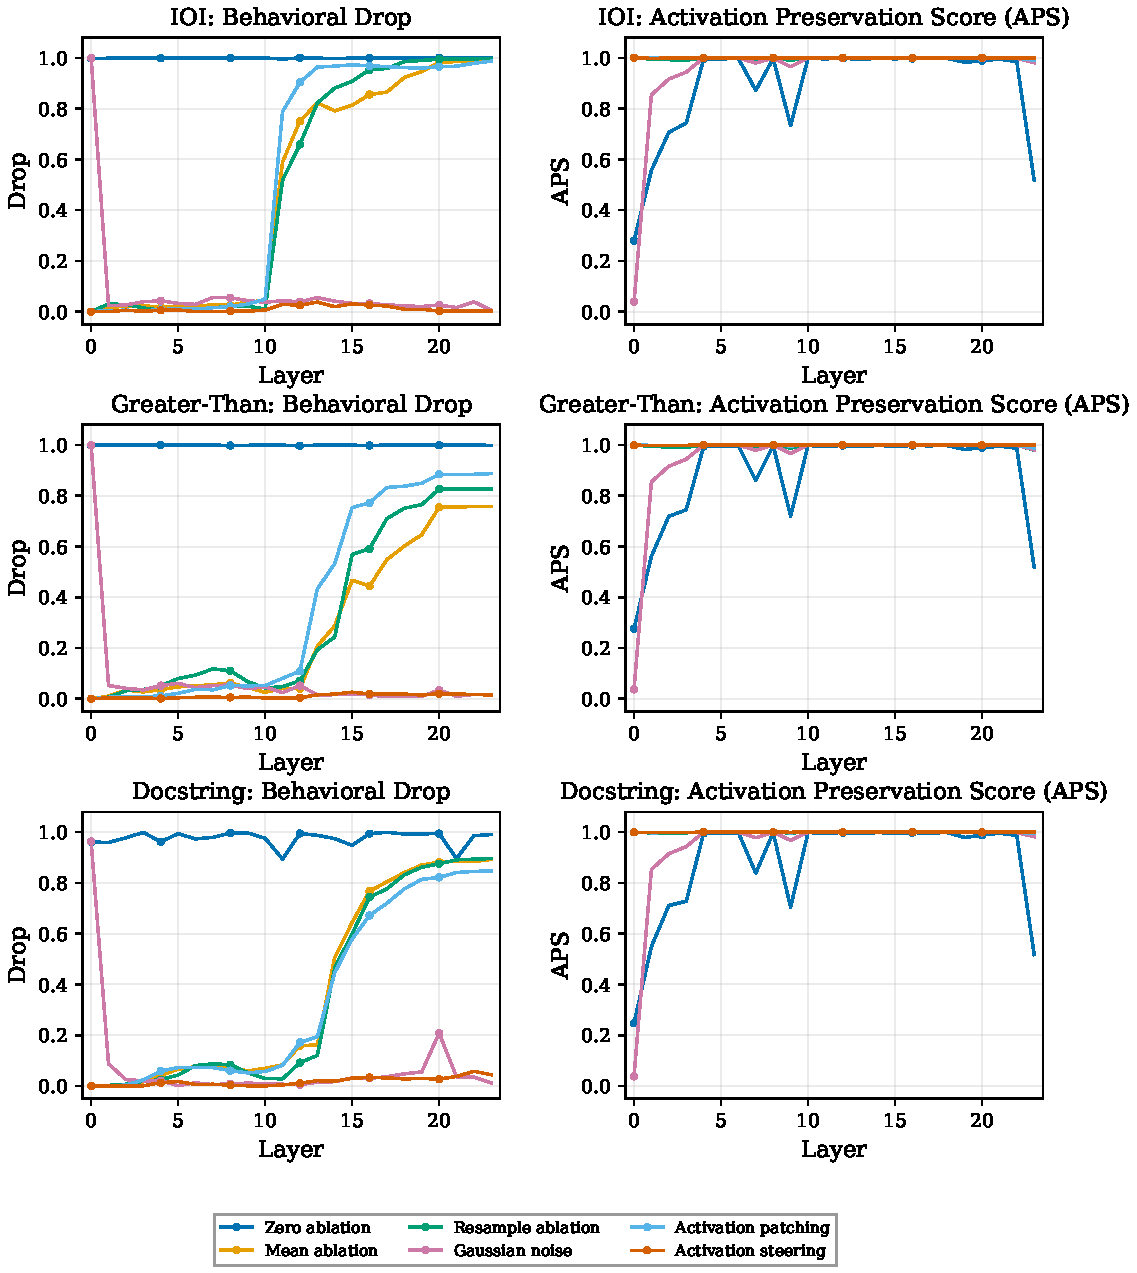
\includegraphics[width=\textwidth]{figures/intervention_comparison.pdf}
\caption{Behavioral drop (left column) and Activation Preservation Score (APS, right column) across layers for IOI (top), Greater-Than (middle), and Docstring (bottom) circuits on Pythia-1.4B. Six intervention methods are compared: zero ablation, mean ablation, resample ablation, Gaussian noise injection, activation patching, and activation steering. APS = 1 indicates perfect preservation of the activation distribution; APS = 0 indicates complete disruption.}
\label{fig:comparison}
\end{figure}

\section{Discussion}
\label{sec:discussion}

\subsection{Guidelines for Method Selection}

Based on our analysis and experimental validation, we provide actionable guidelines:

\begin{enumerate}
    \item \textbf{Use ablation for necessity checks only.} Ablation remains the simplest method when the question is strictly ``Is this component necessary?'' For sufficiency questions, use activation patching.
    \item \textbf{Prefer steering for cost-sensitive settings.} Activation steering provides a computationally efficient screening pass with moderate correlation to ablation conclusions ($\tau \approx 0.45$).
    \item \textbf{Cross-validate key findings.} If ablation is the primary method, validate key conclusions with at least one alternative method (steering or noise injection).
    \item \textbf{Report representational health metrics.} Include Activation Preservation Score or a similar diagnostic alongside behavioral metrics to avoid measurement-behavior mismatch.
    \item \textbf{Test across tasks and scales.} Validate conclusions on at least two different tasks and, where possible, on at least one additional model scale before claiming generality.
\end{enumerate}

\subsection{Limitations}

Our taxonomy is qualitative; formalizing the dimensions as a metric space is future work. Method mappings are approximate (steering strength varies continuously, but we treat it as a single point). Our experimental validation, while systematic, is limited to three circuits on two models (Pythia-1.4B and GPT-2 Small). We do not claim ablation is never correct: for simple necessity checks on small models, it remains the simplest and most interpretable method. The cross-model results, while qualitatively consistent, cover only two model scales; larger-scale replication (e.g., on 7B+ parameter models) would further strengthen generality.

\subsection{A Call to Action}

\begin{enumerate}
    \item Adopt an intervention ontology. Justify why an intervention method is appropriate for the causal question.
    \item Cross-validate ablation findings with steering or noise injection.
    \item Report computational cost (forward passes or GPU hours) alongside results.
    \item Include representational health metrics (e.g., Activation Preservation Score) alongside behavioral metrics.
\end{enumerate}

%%%%%%%%%%%%%%%%%%%%%%%%%%%%%%%%%%%%%%%%%%%%%%%%%%
\section{Conclusion}
\label{sec:conclusion}

We have shown that the MI community suffers from an ``ablation bias'': treating a single boundary point of a continuous intervention space as the universal tool for causal analysis. Drawing on evidence from diverse areas of MI, we identified recurring structural limitations of ablation. We proposed a formal three-dimensional intervention space and experimentally demonstrated substantial method disagreement (mean Kendall $\bar\tau = -0.10$) and that zero ablation over-reports component importance by 85\% compared to mean ablation, with cross-model validation confirming these findings on GPT-2 Small. We urge the community to adopt a richer, more principled approach to intervention method selection.

%%%%%%%%%%%%%%%%%%%%%%%%%%%%%%%%%%%%%%%%%%%%%%%%%%
\section*{Acknowledgements}

We thank the reviewers for their constructive feedback, which has substantially improved the methodological rigor of this work.

\section*{CRediT authorship contribution statement}
\textbf{Dong Liu:} Conceptualization, Methodology, Software, Formal analysis, Investigation, Writing -- original draft, Writing -- review \& editing, Visualization. \textbf{Caihuan Zhang:} Validation, Writing -- review \& editing, Supervision.

\section*{Declaration of competing interest}
The authors declare that they have no known competing financial interests or personal relationships that could have appeared to influence the work reported in this paper.

\section*{Data availability}
The experimental data and analysis code are available at \url{https://github.com/lyld3618/sparse-intervention}. The Pythia-1.4B model~\cite{Biderman2023} and GPT-2 Small are publicly available.

%%%%%%%%%%%%%%%%%%%%%%%%%%%%%%%%%%%%%%%%%%%%%%%%%%
%% Bibliography
\bibliography{references}

\end{document}
